\subsection{Auswirkung der verschiedenen Verfahren}
Um die einzelnen Verfahren besser Vergleichen zu können wurden künstliche Augen aus dem Datensatz \cite{database_Eye} verwendet, damit die exakte Position der Landmarks bekannt ist.\\
Ein gutes Verfahren muss stabil gegenüber der Skalierung sein damit es auch auf kleinen Bereichen zuverlässig arbeitet. Da für die spätere Anwendung vor allem das Zentrum der Pupille von Interesse ist, wird der Abstand zum Zentrum als Qualitätsmaß verwendet.\\
Da auch in der späteren Anwendung der Augenbereich genauer bestimmt ist, als in den Bildern dargestellt, wurde der Bildbereich soweit verkleinert damit noch alle Landmarks des Auges mit etwas Rand in diesem liegen. Somit sind die Bildausschnitten auf denen gerechnet wird etwa 64 auf 29 Pixel groß und werden für die Verarbeitung auf eine Breite von 384 Pixeln vergrößert. Um die Qualität der Berechnung bei verschiedenen Größen zu simulieren, wurde das Bild linear verkleinert.\\
\begin{figure}
	\centering
	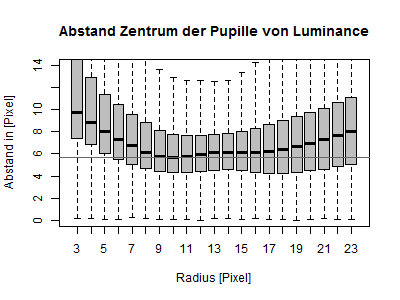
\includegraphics[width=0.32\linewidth]{Eye_Img_Box/Norm_Radius_A}
	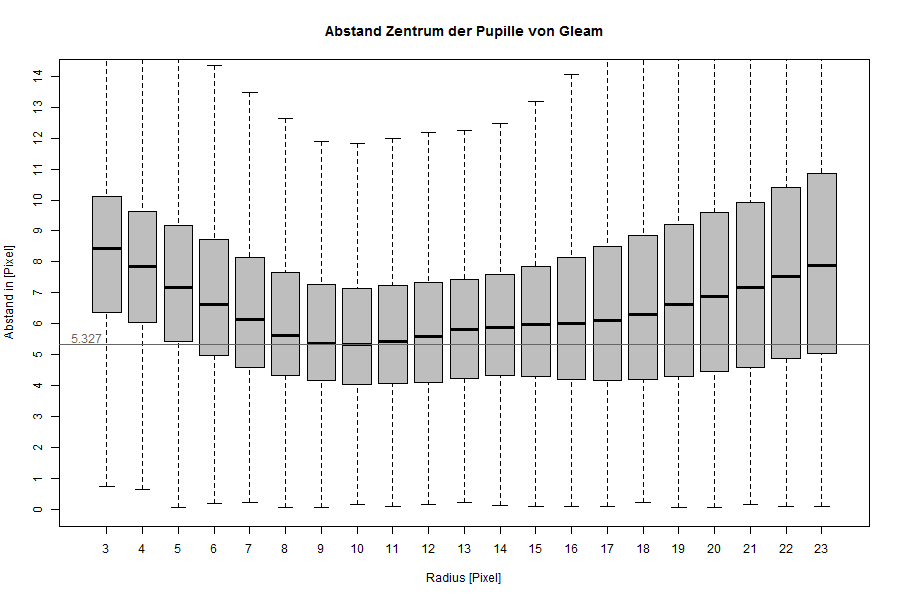
\includegraphics[width=0.32\linewidth]{Eye_Img_Box/Gleam_Radius_A}
	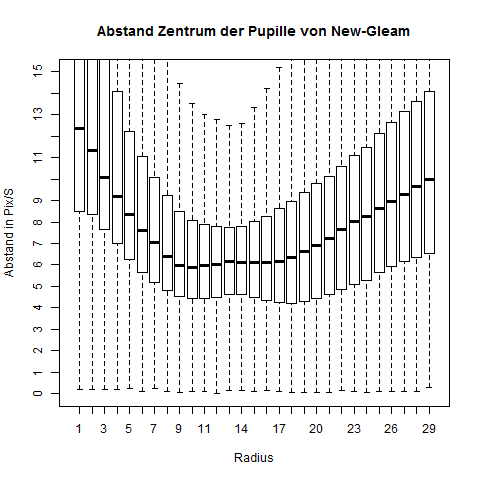
\includegraphics[width=0.32\linewidth]{Eye_Img_Box/New_Radius_A}
	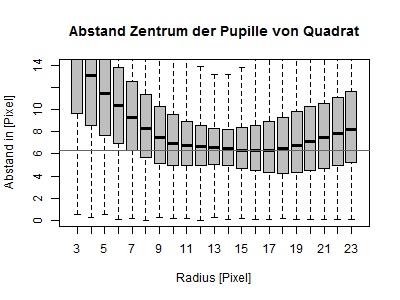
\includegraphics[width=0.32\linewidth]{Eye_Img_Box/Qua_Radius_A}
	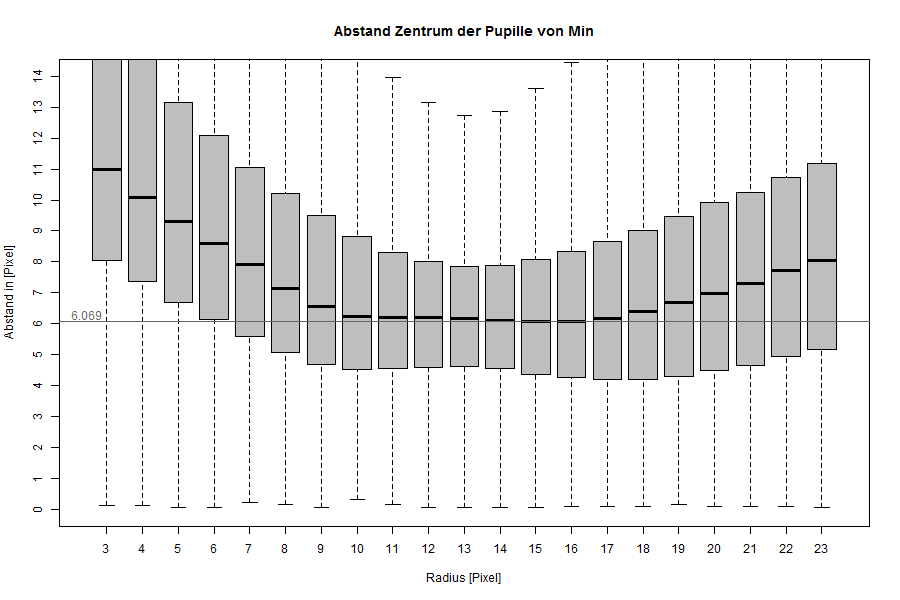
\includegraphics[width=0.32\linewidth]{Eye_Img_Box/Min_Radius_A}
	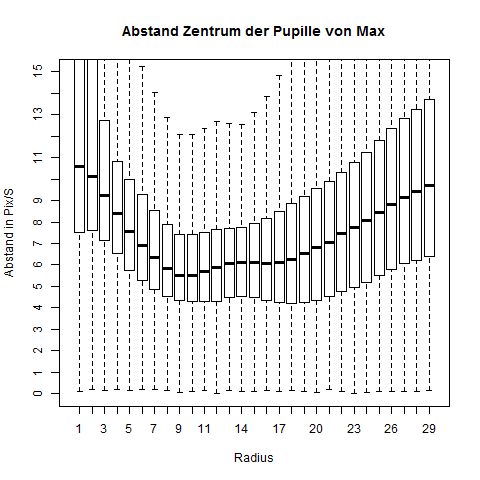
\includegraphics[width=0.32\linewidth]{Eye_Img_Box/Max_Radius_A}
	%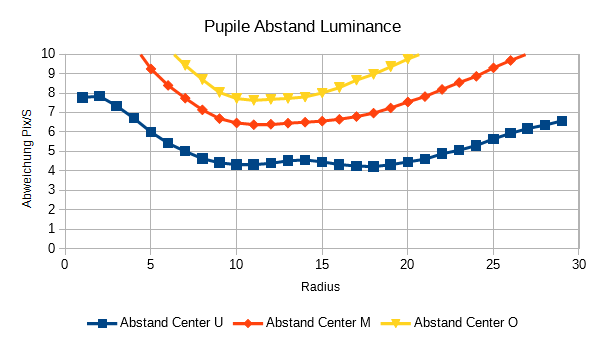
\includegraphics[width=0.49\linewidth]{Eye_Img/Normal_Abstand_P}
	%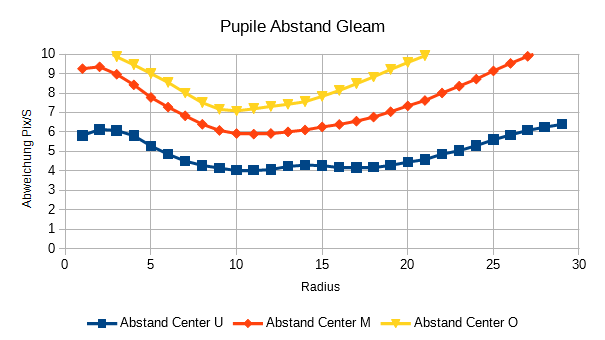
\includegraphics[width=0.49\linewidth]{Eye_Img/Gleam_Abstand_P}
	%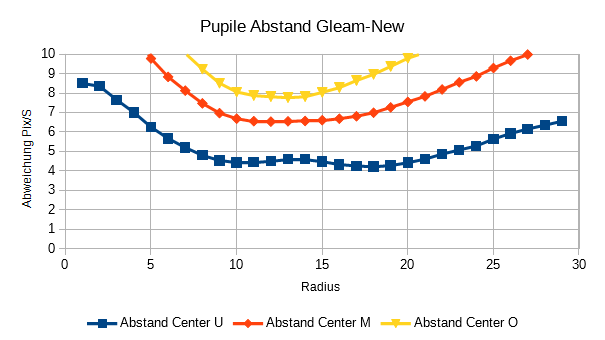
\includegraphics[width=0.49\linewidth]{Eye_Img/New_Abstand_P}
	%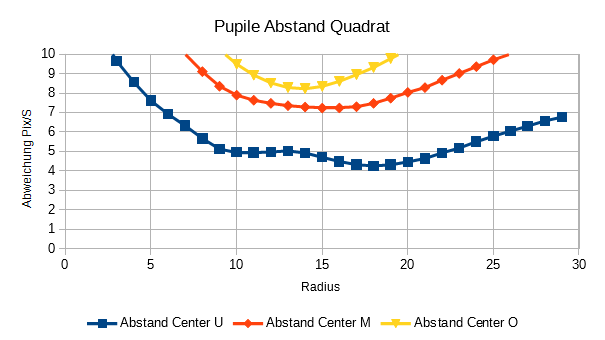
\includegraphics[width=0.49\linewidth]{Eye_Img/Quadrat_Abstand_P}
	%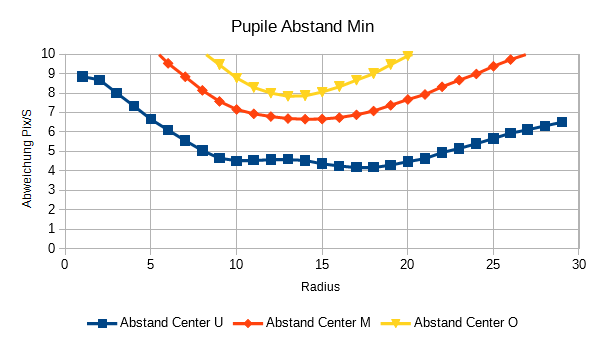
\includegraphics[width=0.49\linewidth]{Eye_Img/Min_Abstand_P}
	%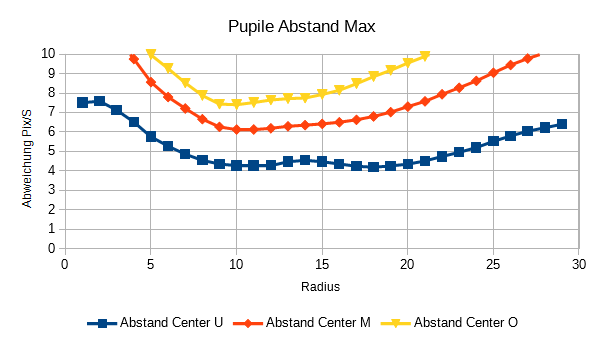
\includegraphics[width=0.49\linewidth]{Eye_Img/Max_Abstand_P}
	\caption{Abstand des Zentrums der Landmark-Pupille und der berechneten Ellipse in [Pixel/Skalierung]\\Oben-Links: Luminance, Oben-Mitte: Gleam, Oben-Rechts: Gleam New, Unten-Links: Quadrat, Unten-Mitte: Min-Wert, Unten-Rechts: Max-Wert}
	\label{ElSe_Gray_Zentrum}
\end{figure}
\begin{figure}
	\centering
	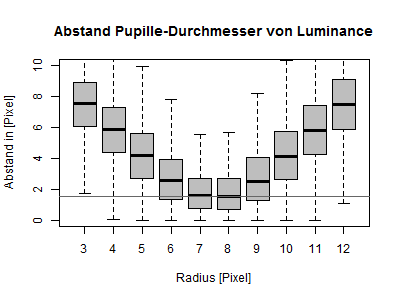
\includegraphics[width=0.32\linewidth]{Eye_Img_Box/Norm_Radius_P}
	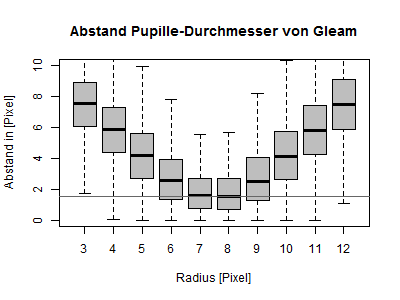
\includegraphics[width=0.32\linewidth]{Eye_Img_Box/Gleam_Radius_P}
	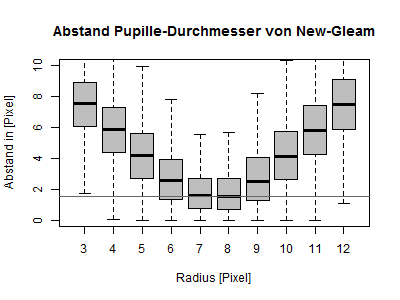
\includegraphics[width=0.32\linewidth]{Eye_Img_Box/New_Radius_P}
	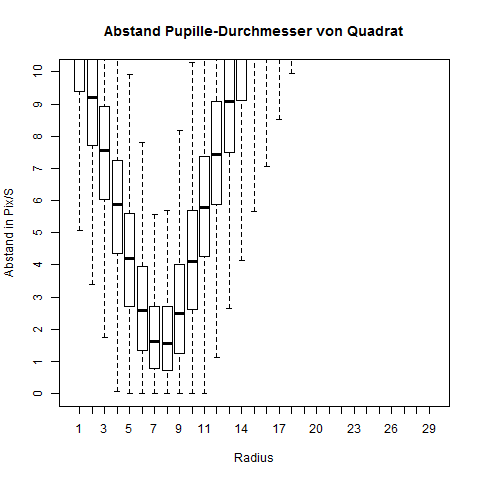
\includegraphics[width=0.32\linewidth]{Eye_Img_Box/Qua_Radius_P}
	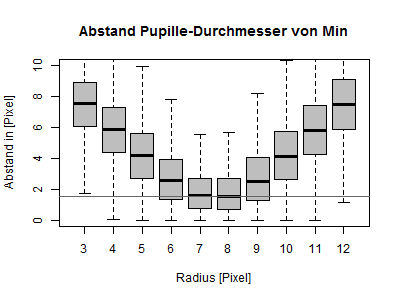
\includegraphics[width=0.32\linewidth]{Eye_Img_Box/Min_Radius_P}
	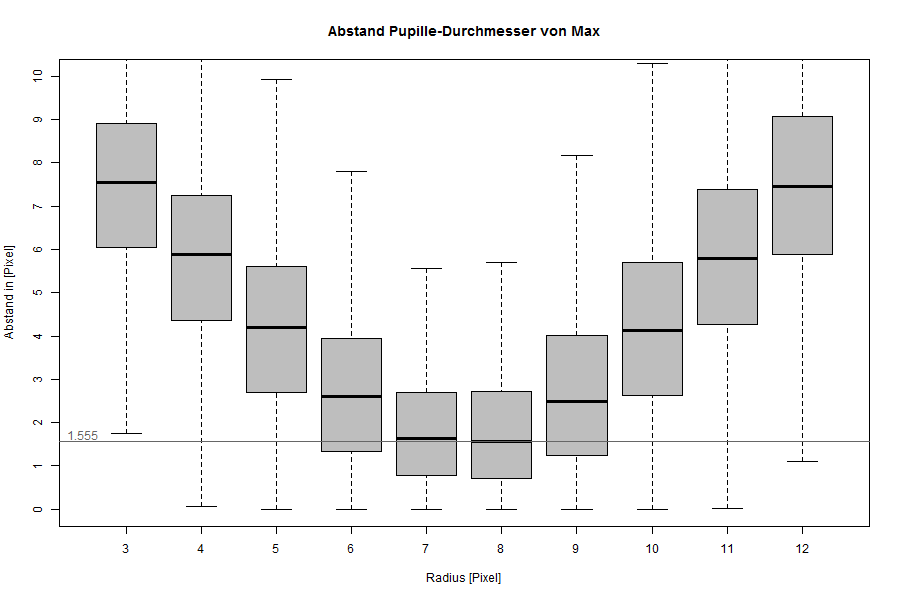
\includegraphics[width=0.32\linewidth]{Eye_Img_Box/Max_Radius_P}
	%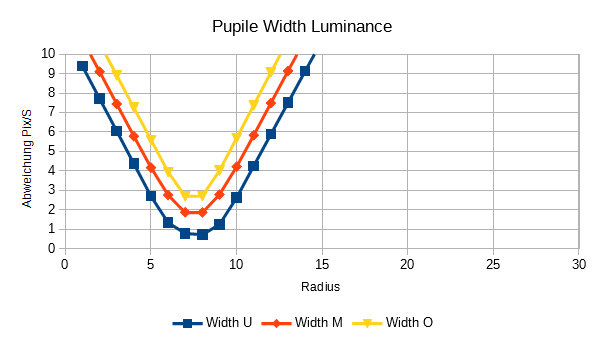
\includegraphics[width=0.49\linewidth]{Eye_Img/Normal_Width_P}
	%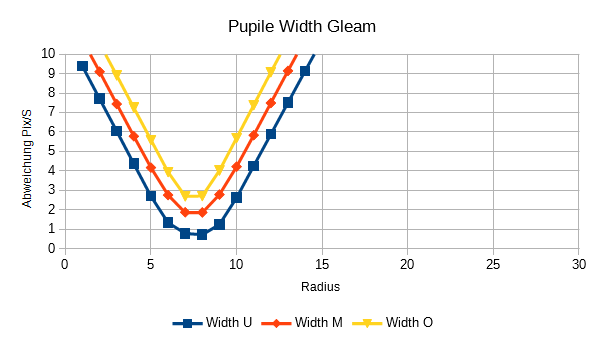
\includegraphics[width=0.49\linewidth]{Eye_Img/Gleam_Width_P}
	%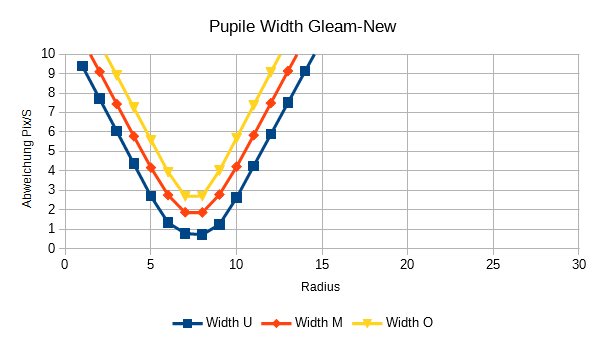
\includegraphics[width=0.49\linewidth]{Eye_Img/New_Width_P}
	%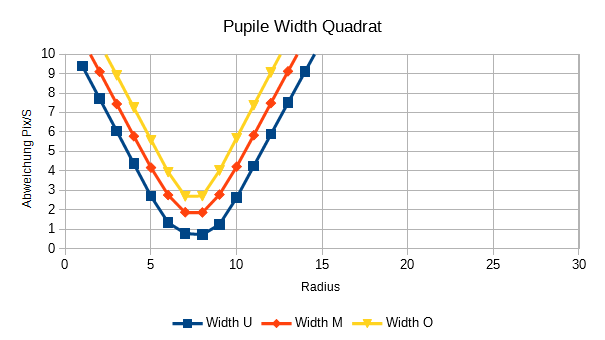
\includegraphics[width=0.49\linewidth]{Eye_Img/Quadrat_Width_P}
	%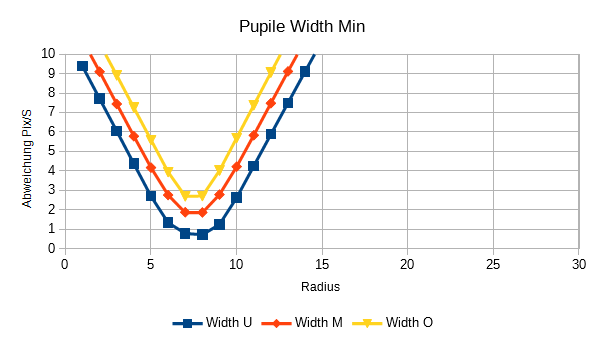
\includegraphics[width=0.49\linewidth]{Eye_Img/Min_Width_P}
	%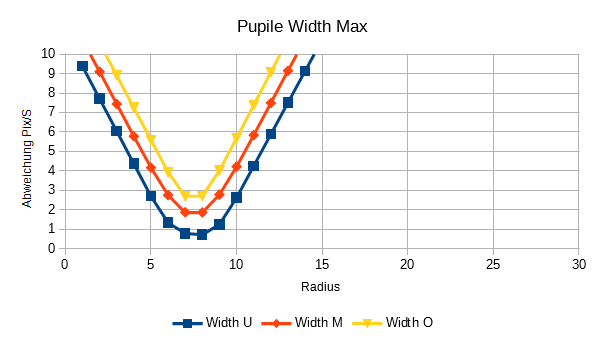
\includegraphics[width=0.49\linewidth]{Eye_Img/Max_Width_P}
	\caption{Unterschied Zwischen den Radien der Landmark-Pupille und der Berechneten Ellipse in [Pixel/Skalierung]\\Oben-Links: Luminance, Oben-Mitte: Gleam, Oben-Rechts: Gleam New, Unten-Links: Quadrat, Unten-Mitte: Min-Wert, Unten-Rechts: Max-Wert}
	\label{ElSe_Gray_Pupille}
\end{figure}
\begin{figure}
	\centering
	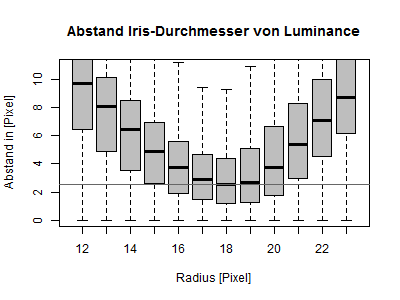
\includegraphics[width=0.32\linewidth]{Eye_Img_Box/Norm_Radius_I}
	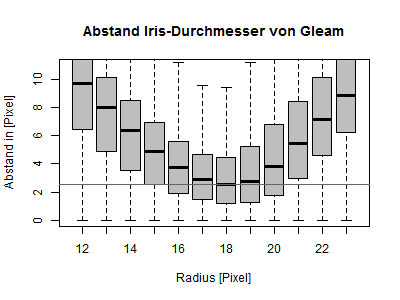
\includegraphics[width=0.32\linewidth]{Eye_Img_Box/Gleam_Radius_I}
	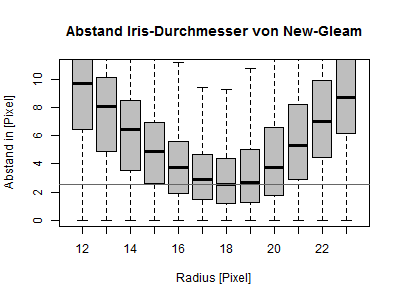
\includegraphics[width=0.32\linewidth]{Eye_Img_Box/New_Radius_I}
	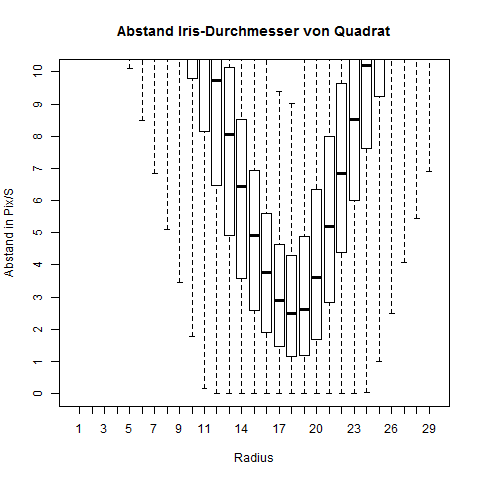
\includegraphics[width=0.32\linewidth]{Eye_Img_Box/Qua_Radius_I}
	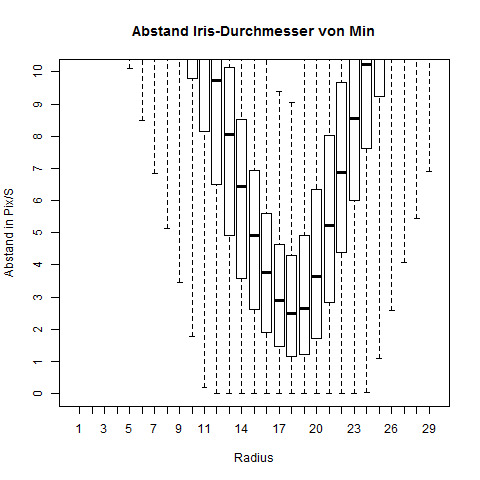
\includegraphics[width=0.32\linewidth]{Eye_Img_Box/Min_Radius_I}
	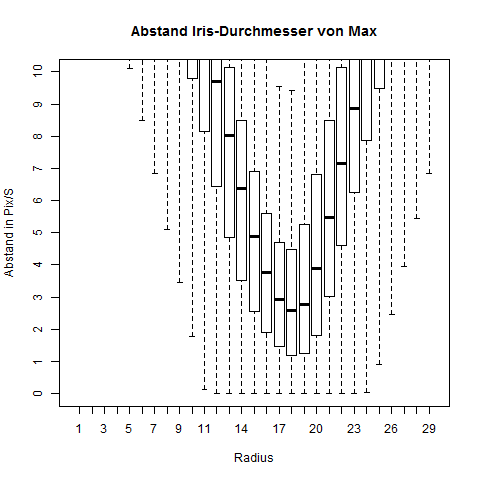
\includegraphics[width=0.32\linewidth]{Eye_Img_Box/Max_Radius_I}
	%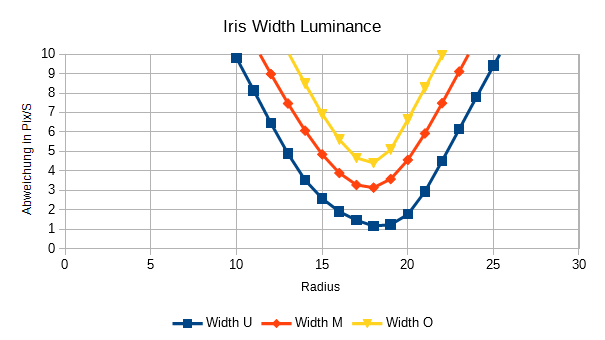
\includegraphics[width=0.49\linewidth]{Eye_Img/Normal_Width_I}
	%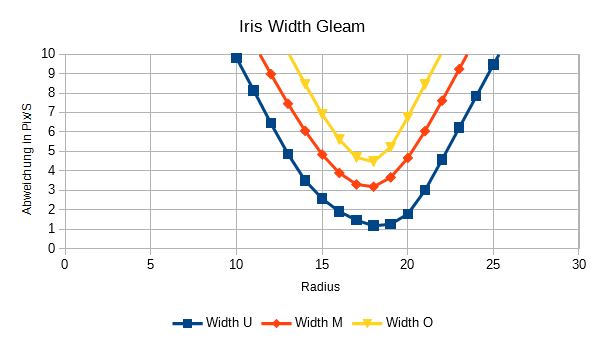
\includegraphics[width=0.49\linewidth]{Eye_Img/Gleam_Width_I}
	%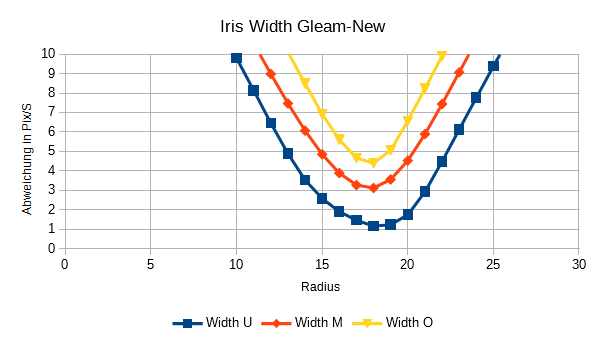
\includegraphics[width=0.49\linewidth]{Eye_Img/New_Width_I}
	%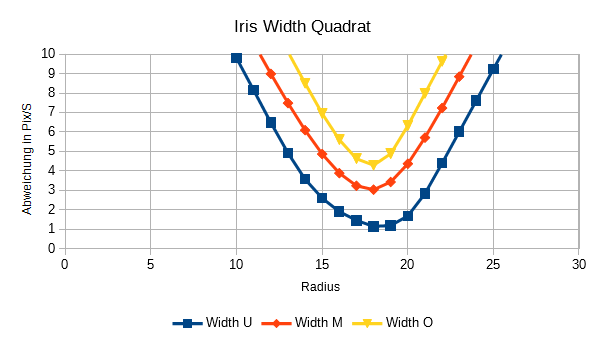
\includegraphics[width=0.49\linewidth]{Eye_Img/Quadrat_Width_I}
	%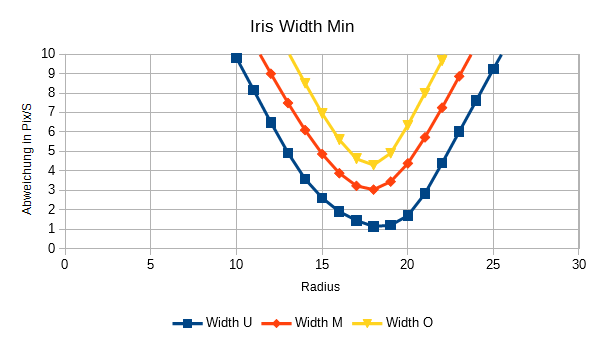
\includegraphics[width=0.49\linewidth]{Eye_Img/Min_Width_I}
	%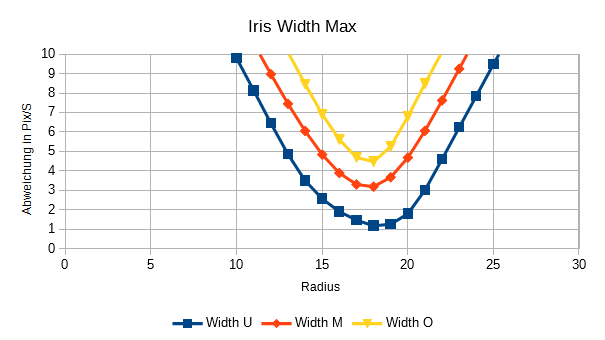
\includegraphics[width=0.49\linewidth]{Eye_Img/Max_Width_I}
	\caption{Unterschied Zwischen den Radien der Landmark-Iris und der Berechneten Ellipse in [Pixel/Skalierung] gegen die Radius-Größe.\\ Oben-Links: Luminance, Oben-Mitte: Gleam, Oben-Rechts: Gleam New, Unten-Links: Quadrat, Unten-Mitte: Min-Wert, Unten-Rechts: Max-Wert}
	\label{ElSe_Gray_Iris}
\end{figure}
Es zeigt sich, dass das Verfahren um den Farbwert in einen Grauwert zu überführen durchaus Auswirkungen auf die Berechnung hat.\\
Es sind Unterschiede zwischen den einzelnen Verfahren zu erkennen. Das beste Ergebnis liefert das Gleab-Verfahren (Beschreiben in \autoref{gray_Gleam}) heraus mit einer Abweichung von 5.89 Pixeln, siehe \autoref{ElSe_Gray_Zentrum}, da die Abweichung vom Zentrum minimal ist. Ein mittleres Ergebnis liefert das Luminance-Verfahren, beschreiben in \autoref{gray_Luminance}, mit welchem eine Abweichung auf dem Augen-Trainingsdatensatz von 6.42 Pixel erreicht wird.\\
Im Vergleich liefert das Quadratische-Verfahren, beschreiben in \autoref{gray_Quadrat} hat im Test die schlechtesten Ergebnis, da die durchschnittliche Abweichung bei 7.23 Pixel liegt.\\
\begin{figure}
	\centering
	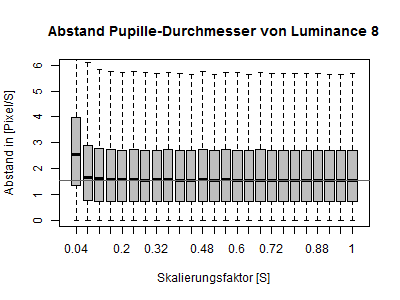
\includegraphics[width=0.32\linewidth]{Eye_Img_Box/Norm_Radius_P_8}
	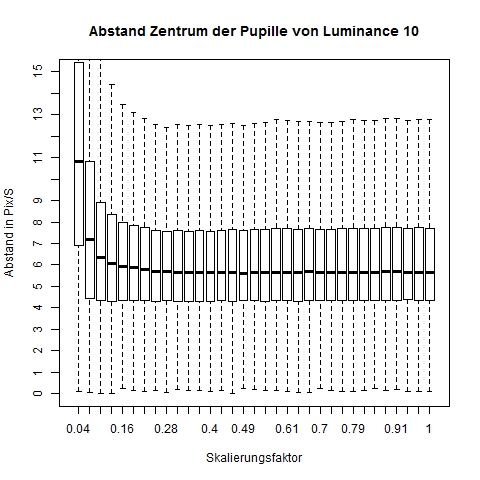
\includegraphics[width=0.32\linewidth]{Eye_Img_Box/Norm_Radius_A_10}
	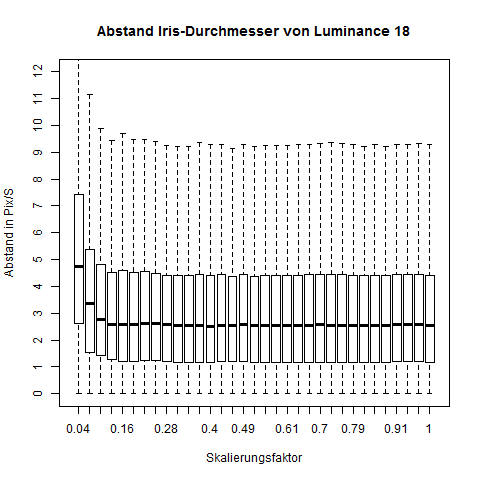
\includegraphics[width=0.32\linewidth]{Eye_Img_Box/Norm_Radius_I_18}\\
	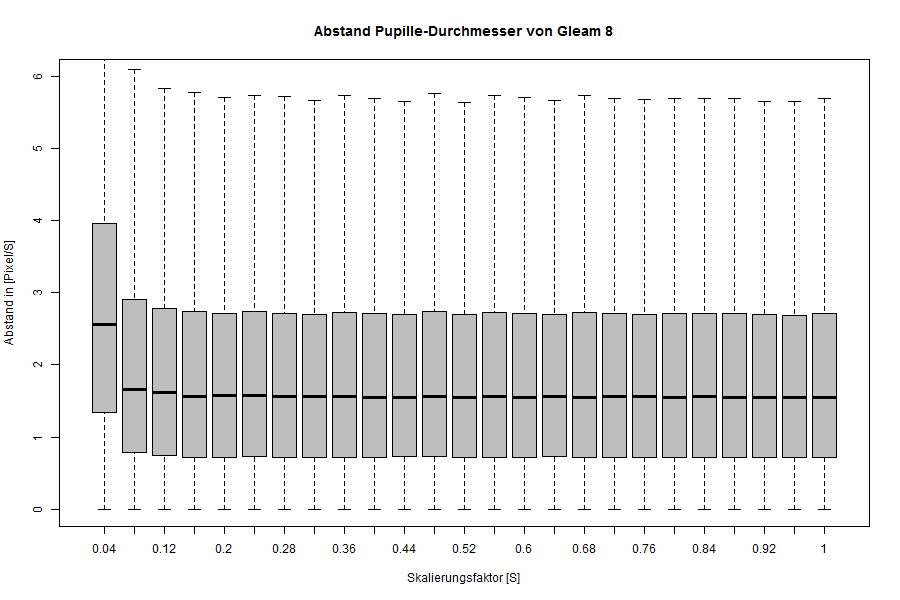
\includegraphics[width=0.32\linewidth]{Eye_Img_Box/Gleam_Radius_P_8}
	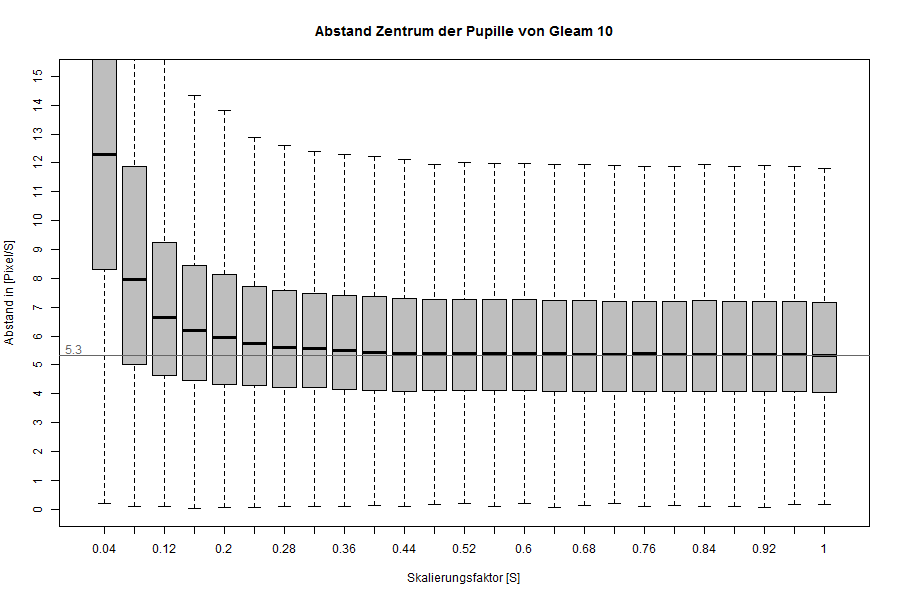
\includegraphics[width=0.32\linewidth]{Eye_Img_Box/Gleam_Radius_A_10}
	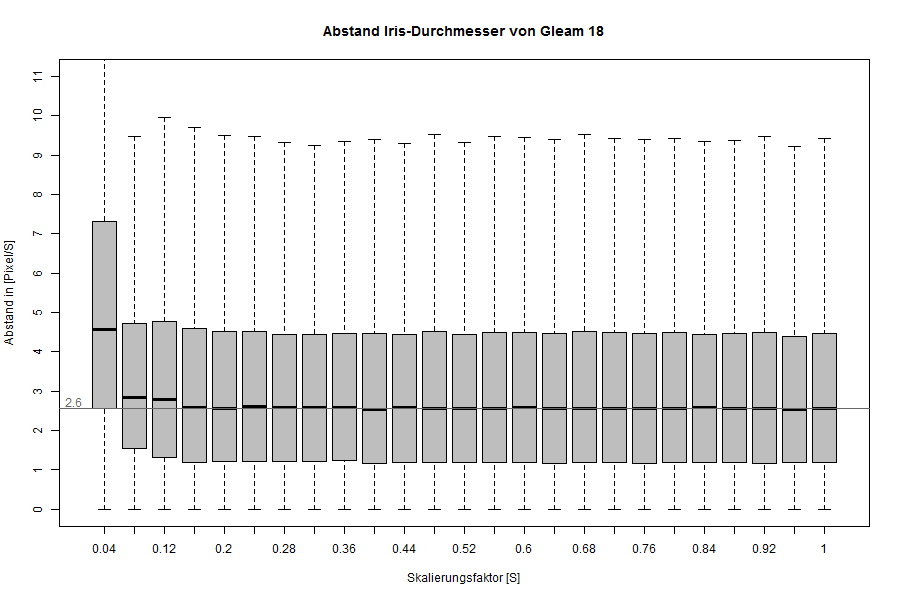
\includegraphics[width=0.32\linewidth]{Eye_Img_Box/Gleam_Radius_I_18}
	%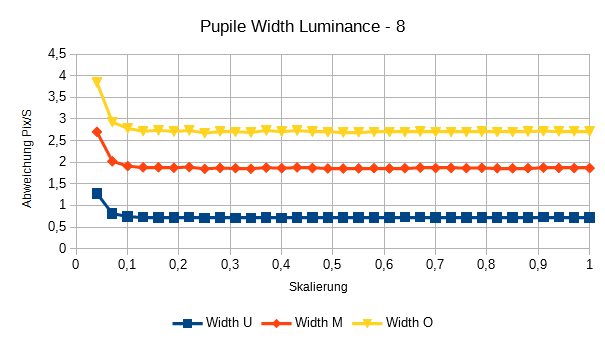
\includegraphics[width=0.32\linewidth]{Eye_Img/Normal_Width_P_8}
	%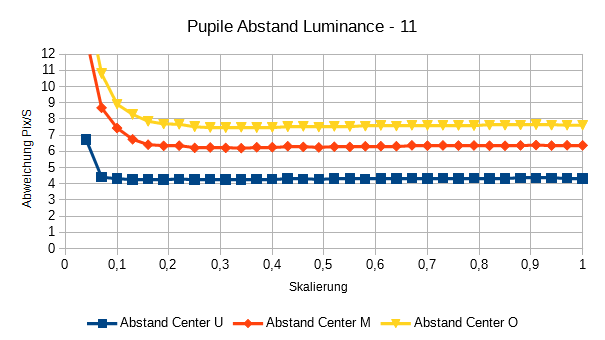
\includegraphics[width=0.32\linewidth]{Eye_Img/Normal_Abstand_P_11}
	%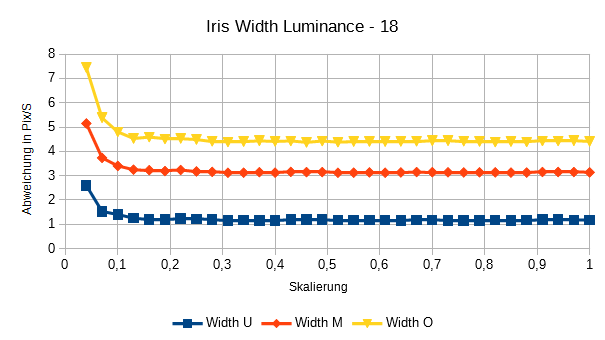
\includegraphics[width=0.32\linewidth]{Eye_Img/Normal_Width_I_18}\\
	%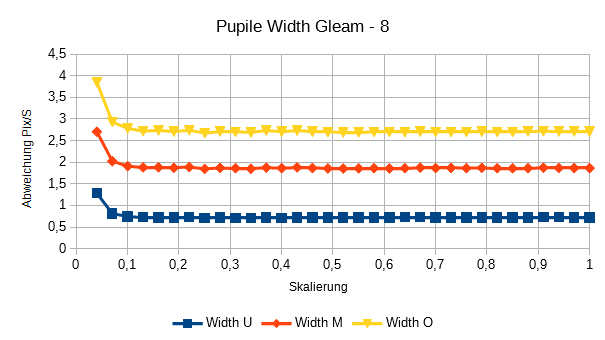
\includegraphics[width=0.32\linewidth]{Eye_Img/Gleam_Width_P_8}
	%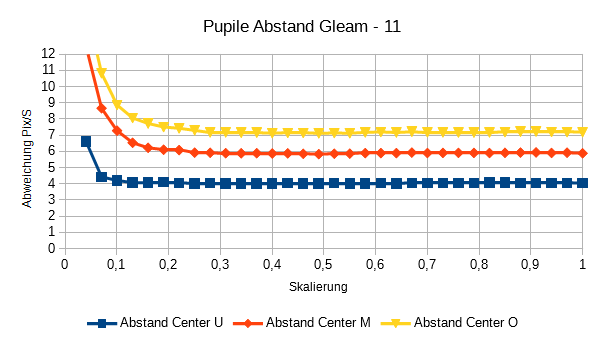
\includegraphics[width=0.32\linewidth]{Eye_Img/Gleam_Abstand_P_11}
	%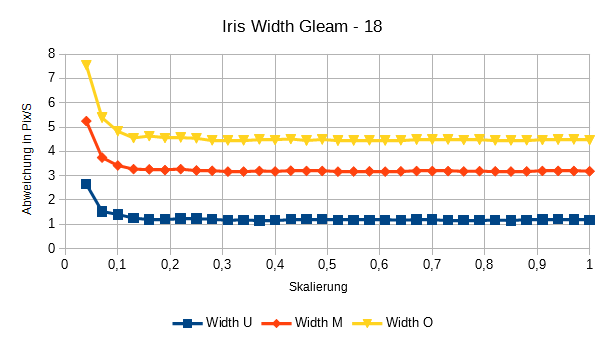
\includegraphics[width=0.32\linewidth]{Eye_Img/Gleam_Width_I_18}
	\caption{Auswirkung von der Bildgröße auf die Qualität der Berechnung.\\ Oben: Luminance, Unten Gleam}
	\label{ElSe_scall}
\end{figure}
Bei der Berechnung auf verscheiden groß skalierten Bildern ist die Abweichung von ElSe bei Verwendung von Gleam konstant bei etwa 5.9 Pixel und arbeitet somit stabil, siehe \autoref{ElSe_scall}.\\
So ist im Test der Durchschnitt bei allen Skalierungen ElSe den Ergebnisse von OpenFace überlegen, durch die Verteilung ist allerdings eine Kombination beider Verfahren sinnvoll, so kann das Ergebnis von OpenFace bei Bilder in denen die Iris größer als 21 Pixel ist direkt als Lösung verwendet werden, da der mögliche Fehler von OpenFace geringer ist als von ElSe.\\
Im Bereich zwischen 21 und 15 Pixel können beide Ergebnisse Kombiniert werden, da sie ungefähr gleich gute Ergebnisse liefern.\\
Sollte die Iris im Originalbild noch kleiner sein, so ist ElSe deutlich genauer, da es noch bis zu einer Irisgröße von 3 Pixel noch stabil funktioniert.
\subsection{ElSe - Auswirkung des Radius}
Ein weiter wichtiger Parameter des ElSe-Verfahrens ist der Radius des Filters. Wiederrum wurde der Augen-Datensatz \cite{database_Eye} verwendet und die Augenpartie ausgeschnitten. Im Datensatz besitzen die abgebildeten Augen eine Durchschnittlich Pupille von 15 Pixel und eine Iris von 34 Pixel.\\
In \autoref{ElSe_Gray_Iris} und \autoref{ElSe_Gray_Zentrum} ist zu erkennen, dass die Wahl des Radius signifikant für die Qualität der Berechnung ist. Da für die spätere Anwendung vor allem das Zentrum der Pupille von Interesse ist, siehe \autoref{OpenFace_Blickrichtung}, muss ElSe in diesem Aspekt zuverlässig Ergebnisse liefern.\\
Im Versuch hat sich ein Radius von etwa einem Zwölftel des zu erwartetem Durchmesser der Iris bzw. Pupille als sinnvoll erwiesen, um deren Dimension möglichst exakt zu bestimmen. Im Versuch entspricht dies 8 und 18 Pixel. Um die Position des Zentrums  der Iris und der Pupille möglichst gut zu bestimmen, erwies sich ein Radius von 10 am besten, siehe \autoref{ElSe_Gray_Zentrum}, wobei dieser Fehler nicht so sehr steigt bei Veränderung des Radius, als bei der Größenbestimmung von Pupille und Iris.
\subsection{OpenFace}
Als Referenz wird das Ergebnis von OpenFace für die zusätzlich bestimmten Landmarks der Augen verwendet. Dies wurde auch auf dem Augendatensatz \cite{database_Eye} angewendet um vergleichbare Ergebnisse zu erhalten.\\
Es ist zu erkennen dass dieses Verfahren im Schnitt oft schlechtere Ergebnisse liefert als das Ergebnis von ElSe, allerdings ohne das begehen von großen Fehlern und auch öfters genauere Ergebnisse.\\
Da die hohe Qualität von ElSe nur erreicht werden kann, wenn es auf den passenden Bildausschnitt angewendet wird, ist auch die Detektion des Auge von Interesse.\\
Nach \autoref{OpenFace_Eye_Box} wird der Bereich des Auges zwar nicht so exakt bestimmt, allerdings überdeckt er den relevanten Bereich ausreichend genau. Dargestellt sind Koordinaten, X- und Y-Position in Pixel sowie die Ausdehnung, Width und Hight bestenfalls in Pixel relativ zur umschließenden Box der Landmarks. Somit liegen die Landmarks der Augen im Bildausschnitt, wodurch diese Ausschnitt verwendet werden kann als Eingabe von ElSe.
\begin{figure}
	\centering
	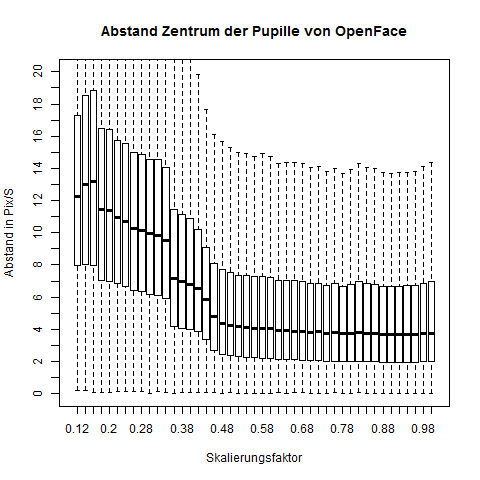
\includegraphics[width=0.45\linewidth]{Eye_Img_Box/Openface_PC}
	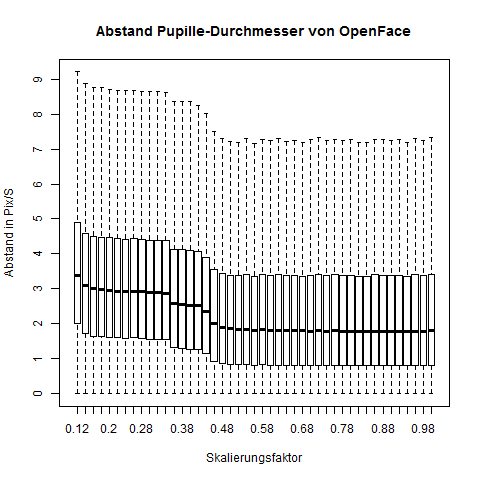
\includegraphics[width=0.45\linewidth]{Eye_Img_Box/Openface_PW}
	%\includegraphics[width=0.45\linewidth]{Eye_Img/OpenFace_Zentrum_P}
	%\includegraphics[width=0.45\linewidth]{Eye_Img/OpenFace_Width_P}
	\caption{Auswirkung von Skalierung auf die Qualität der Augendetektion von ObenFace}
	\label{OpenFace_Eye}
\end{figure}
\begin{figure}
	\centering
	\includegraphics[width=0.245\linewidth]{Eye_Img_Box/Openface_BoxX}
	\includegraphics[width=0.245\linewidth]{Eye_Img_Box/Openface_BoxY}
	\includegraphics[width=0.245\linewidth]{Eye_Img_Box/Openface_BoxW}
	\includegraphics[width=0.245\linewidth]{Eye_Img_Box/Openface_BoxH}
	%\includegraphics[width=0.245\linewidth]{Eye_Img/Box_X}
	%\includegraphics[width=0.245\linewidth]{Eye_Img/Box_Y}
	%\includegraphics[width=0.245\linewidth]{Eye_Img/Box_W}
	%\includegraphics[width=0.245\linewidth]{Eye_Img/Box_H}
	\caption{Bestimmung der Box ums Auge}
	\label{OpenFace_Eye_Box}
\end{figure}

